\paragraph{O solo.} As cinco zonas não são camadas: são cinco regiões do morro Umyeon (Fig.~3 do artigo), cada uma
calculada à parte como uma camada homogênea de 2~m de coluvião sobre a rocha (a base impermeável). Os parâmetros
estão na Tab.~\ref{tab:kangparam}: os do artigo (Tabelas~1 e 2) e os que ele não dá (marcados).

\begin{table}[H]\centering\small
\caption{Kang et al.\ (2020): os parâmetros adotados. Por zona, a Tabela~1 do artigo e os ângulos máximo, médio e
mínimo dos taludes rompidos (legenda da Fig.~9). Curvas de van Genuchten ($S_e = [1 + (\psi/P_0)^{n}]^{-m}$,
$m = 1 - 1/n$) do lado norte (zonas 1 e 2) e do sul (3 a 5); $\theta_s$ e $\theta_r$ lidos da Fig.~4a (a porosidade
é $\theta_s$ e $S_{rw} = \theta_r/\theta_s$). $^*$: hipótese nossa (o artigo não dá).}\label{tab:kangparam}
\begin{tabular}{cccccccc}
\toprule
zona & $\phi'$ ($^\circ$) & $c'$ (kPa) & $\gamma_t$ (kN/m$^3$) & $\gamma_d$ (kN/m$^3$) & $k_s$ (m/s) & curva &
$\beta$ máx./méd./mín. ($^\circ$)\\
\midrule
1 & 25,3 & 9,6 & 18,1 & 15,0 & $7{,}15\times10^{-6}$ & norte & 38,8 / 30,7 / 26,5\\
2 & 28,5 & 5,8 & 17,7 & 14,9 & $3{,}87\times10^{-6}$ & norte & 37,4 / 31,0 / 23,3\\
3 & 37,6 & 7,7 & 17,0 & 14,0 & $1{,}80\times10^{-6}$ & sul & 40,5 / 31,2 / 23,3\\
4 & 30,9 & 7,6 & 17,3 & 14,5 & $9{,}70\times10^{-6}$ & sul & 40,5 / 31,8 / 24,8\\
5 & 28,2 & 6,3 & 18,2 & 15,0 & $3{,}69\times10^{-6}$ & sul & 40,3 / 31,1 / 24,7\\
\bottomrule
\end{tabular}

\vspace{2mm}
\begin{tabular}{lcc}
\toprule
curva & norte (zonas 1, 2) & sul (zonas 3, 4, 5)\\
\midrule
$1/P_0$ (1/kPa) & 0,051 & 0,038\\
$m$ ($n$) & 0,35 (1,538) & 0,63 (2,703)\\
$\theta_s$ ($= n$) / $\theta_r$ ($S_{rw}$)$^*$ & 0,50 / 0,19 (0,38) & 0,51 / 0,183 (0,36)\\
\bottomrule
\end{tabular}

\vspace{2mm}
\begin{tabular}{ll}
\toprule
água e ar (Tabela 2) & $\mu_w/\mu_a = 56$; $K_w = 2$~GPa; $\rho_a = 1{,}25$~kg/m$^3$; ar como gás ideal a 101,3~kPa
($K_a \approx 100$~kPa)\\
permeabilidades relativas & $k_{rw}$ de Mualem ($b = 0{,}5$), tabelada perto da saturação no norte$^*$ ($n < 2$);
$k_{ra}$ de Lenhard--Parker ($c = 0{,}5$), piso $10^{-4}$$^*$\\
tensão efetiva & Bishop com $\chi = S_w$; Biot $\alpha = 1$\\
esqueleto$^*$ & elástico, $E = 20$~MPa, $\nu = 0{,}3$; peso $\gamma_t$\\
estado inicial & $p_w = -20$~kPa constante, $p_a = 0$; estado geostático\\
chuva & a Fig.~2 do artigo digitalizada$^*$ (381~mm em 17~h); passo de 0,05~h\\
\bottomrule
\end{tabular}
\end{table}

\paragraph{As duas malhas.} O artigo usa no FLAC uma faixa inclinada de 10~m na horizontal, com laterais verticais de
2~m e $40 \times 20$ zonas (Fig.~5 do artigo). Ela é reproduzida aqui com os mesmos nós, cada zona em quatro triângulos
em volta do centro (Fig.~\ref{fig:kangfaixa}; 16\,364 equações), e o FS é tomado na vertical do meio. A alternativa é a
coluna vertical que a representa no limite 1D (Fig.~\ref{fig:kangmalha}; 1050 equações), vinte vezes mais barata.

\begin{figure}[H]\centering
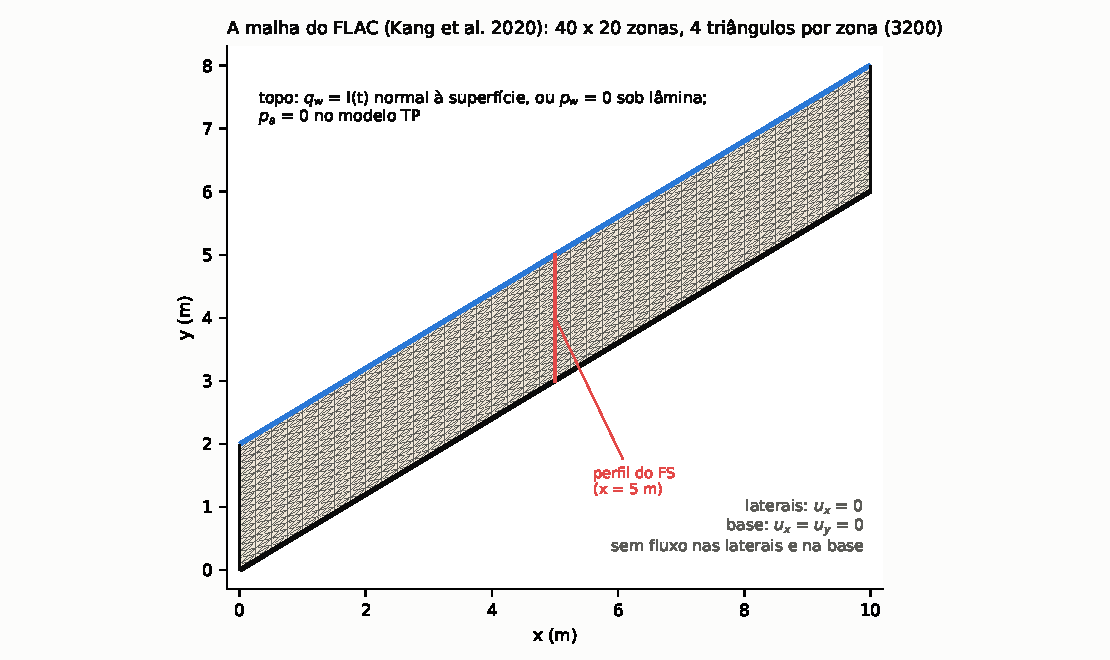
\includegraphics[width=0.9\textwidth]{figs/kang_faixa_malha.pdf}
\caption{Kang et al.\ (2020): a malha do artigo (a faixa do FLAC, $40 \times 20$ zonas de $0{,}25 \times 0{,}1$~m), cada
zona em 4 triângulos; no topo, a chuva normal à superfície ou $p_w = 0$ sob lâmina d'água, e $p_a = 0$ com ar ativo;
laterais com $u_x = 0$, base fixa, sem fluxo nas laterais e na base. Em vermelho, a vertical do FS.}\label{fig:kangfaixa}
\end{figure}

\begin{figure}[H]\centering
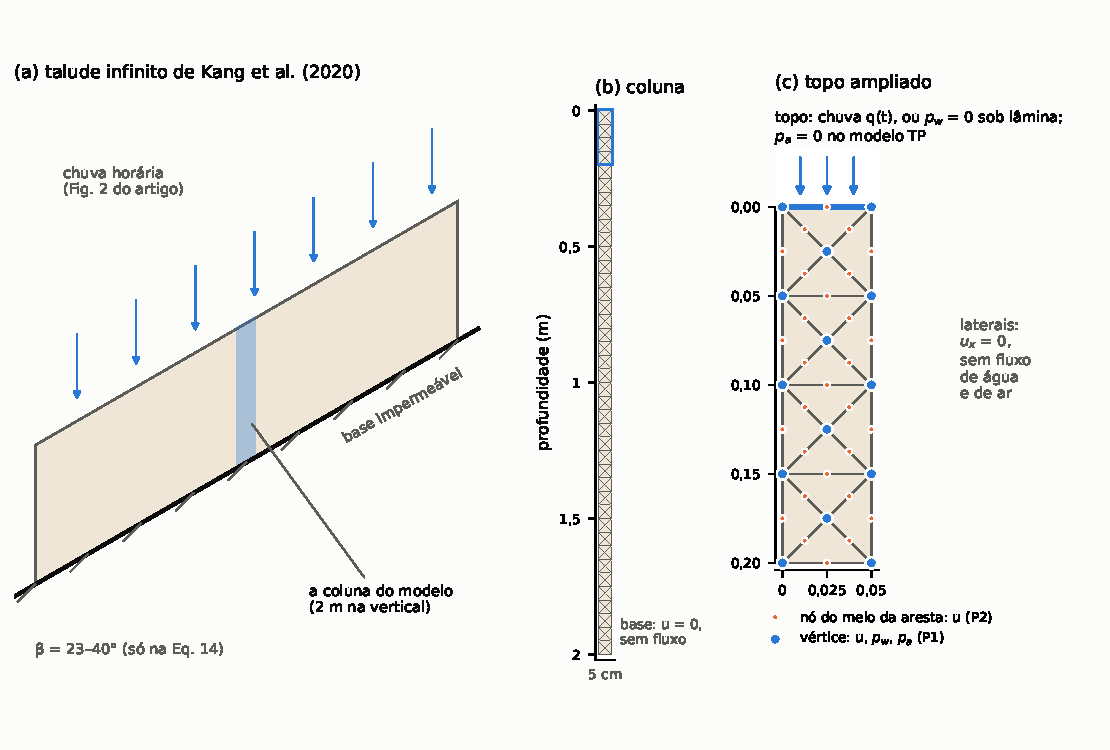
\includegraphics[width=\textwidth]{figs/kang_malha.pdf}
\caption{Kang et al.\ (2020): a coluna. (a) O talude infinito do artigo e a coluna vertical que o representa: o fluxo é
1D na vertical, e o ângulo $\beta$ só entra no FS (Eq.~14). (b) A coluna em escala real, 40 células de 5~cm. (c) O topo
ampliado: 4 triângulos por célula em volta do nó central (malha simétrica), $u$ quadrático e $p_w$, $p_a$ lineares
(Taylor--Hood), 1050 equações; no topo, a chuva ou $p_w = 0$ sob lâmina d'água e $p_a = 0$ no modelo com ar ativo;
laterais e base sem fluxo de água e de ar.}\label{fig:kangmalha}
\end{figure}

\paragraph{Na coluna.} Reproduzidos: no sul (zonas 3--5), a hora em que a coluna satura sem ar, o ``serrote'' do FS
com ar (cai nas horas de chuva forte, recupera nas pausas) e o FS final, com o ar ativo acima do passivo onde o ar fica
preso (zona 3: 1,46 contra 0,83; artigo 1,38 contra 0,79). No norte (zonas 1 e 2) a coluna satura 1--3~h antes do
artigo, provavelmente pela curva de retenção, inconsistente no artigo (Tabela~1 contra Fig.~4a).

\begin{table}[H]\centering\small
\caption{Kang et al.\ (2020), na coluna: FS no ângulo médio de cada zona, nosso / artigo (lido da Fig.~9,
$\pm 0{,}05$).}\label{tab:kang}
\resizebox{\textwidth}{!}{\begin{tabular}{c|cccc|cccc}
\toprule
 & \multicolumn{4}{c|}{TP (ar ativo)} & \multicolumn{4}{c}{SP (ar passivo)}\\
zona & 3~h & 9~h & 12~h & 17~h & 3~h & 9~h & 12~h & 17~h\\
\midrule
1 & 1{,}66 / 1{,}78 & 1{,}60 / 1{,}75 & 1{,}32 / 1{,}55 & 0{,}81 / 0{,}82 & 1{,}76 / 1{,}79 & 1{,}58 / 1{,}76 & 1{,}36 / 1{,}70 & 0{,}81 / 0{,}82 \\
2 & 1{,}62 / 1{,}62 & 1{,}67 / 1{,}66 & 1{,}47 / 1{,}40 & 1{,}24 / 1{,}05 & 1{,}73 / 1{,}77 & 1{,}67 / 1{,}73 & 1{,}56 / 1{,}68 & 0{,}63 / 0{,}62 \\
3 & 1{,}90 / 2{,}05 & 2{,}27 / 2{,}30 & 1{,}62 / 1{,}62 & 1{,}46 / 1{,}38 & 2{,}46 / 2{,}55 & 2{,}35 / 2{,}43 & 2{,}22 / 2{,}30 & 0{,}83 / 0{,}79 \\
4 & 1{,}77 / 1{,}86 & 1{,}55 / 1{,}60 & 0{,}84 / 0{,}85 & 0{,}73 / 0{,}72 & 1{,}83 / 1{,}88 & 1{,}55 / 1{,}60 & 1{,}23 / 1{,}33 & 0{,}73 / 0{,}72 \\
5 & 1{,}32 / 1{,}53 & 1{,}51 / 1{,}55 & 0{,}97 / 0{,}95 & 0{,}74 / 0{,}68 & 1{,}70 / 1{,}75 & 1{,}51 / 1{,}57 & 1{,}36 / 1{,}45 & 0{,}65 / 0{,}60 \\
\bottomrule
\end{tabular}
}
\end{table}

\begin{figure}[H]\centering
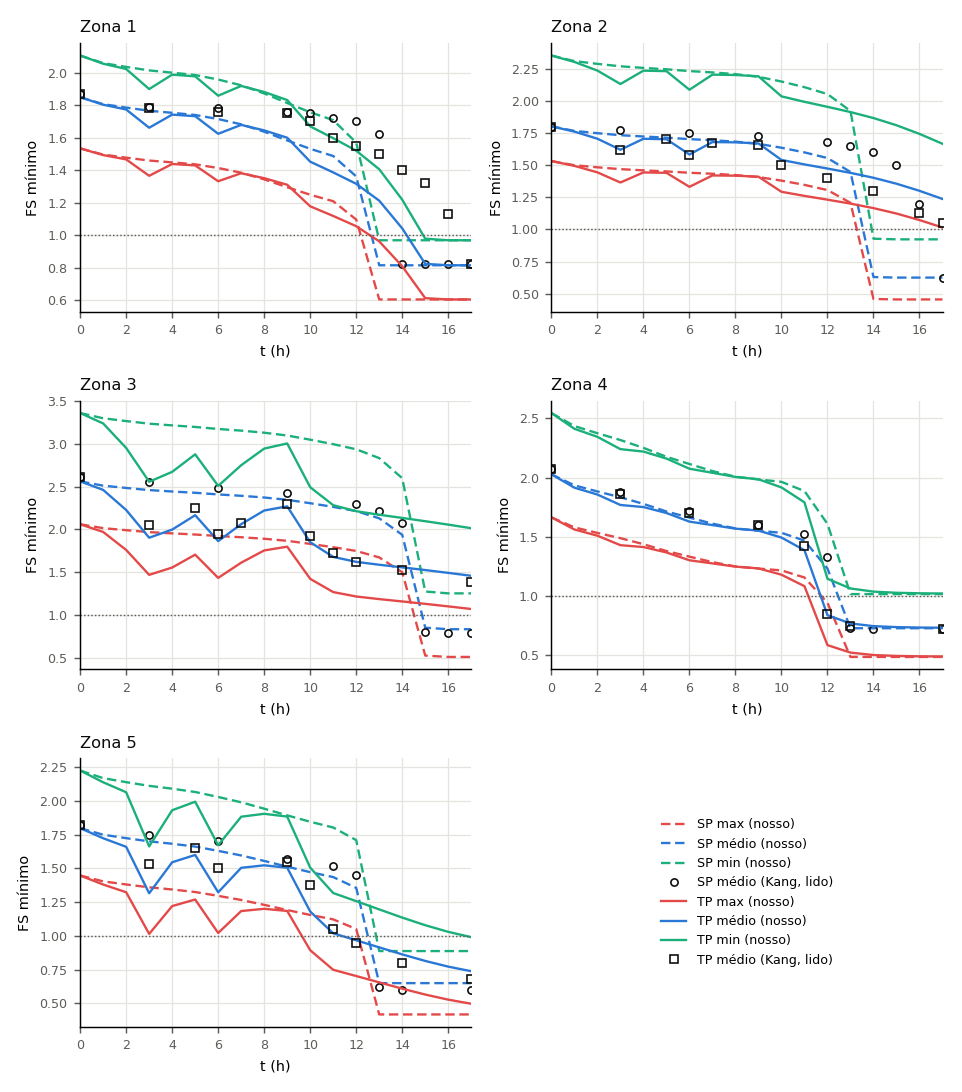
\includegraphics[width=0.9\textwidth]{figs/kang_fig9_nosso.png}
\caption{Kang et al.\ (2020), na coluna: FS mínimo no tempo, nosso (linhas; SP tracejado, TP cheio) e o do artigo no
ângulo médio (marcadores).}\label{fig:kang9}
\end{figure}

\begin{figure}[H]\centering
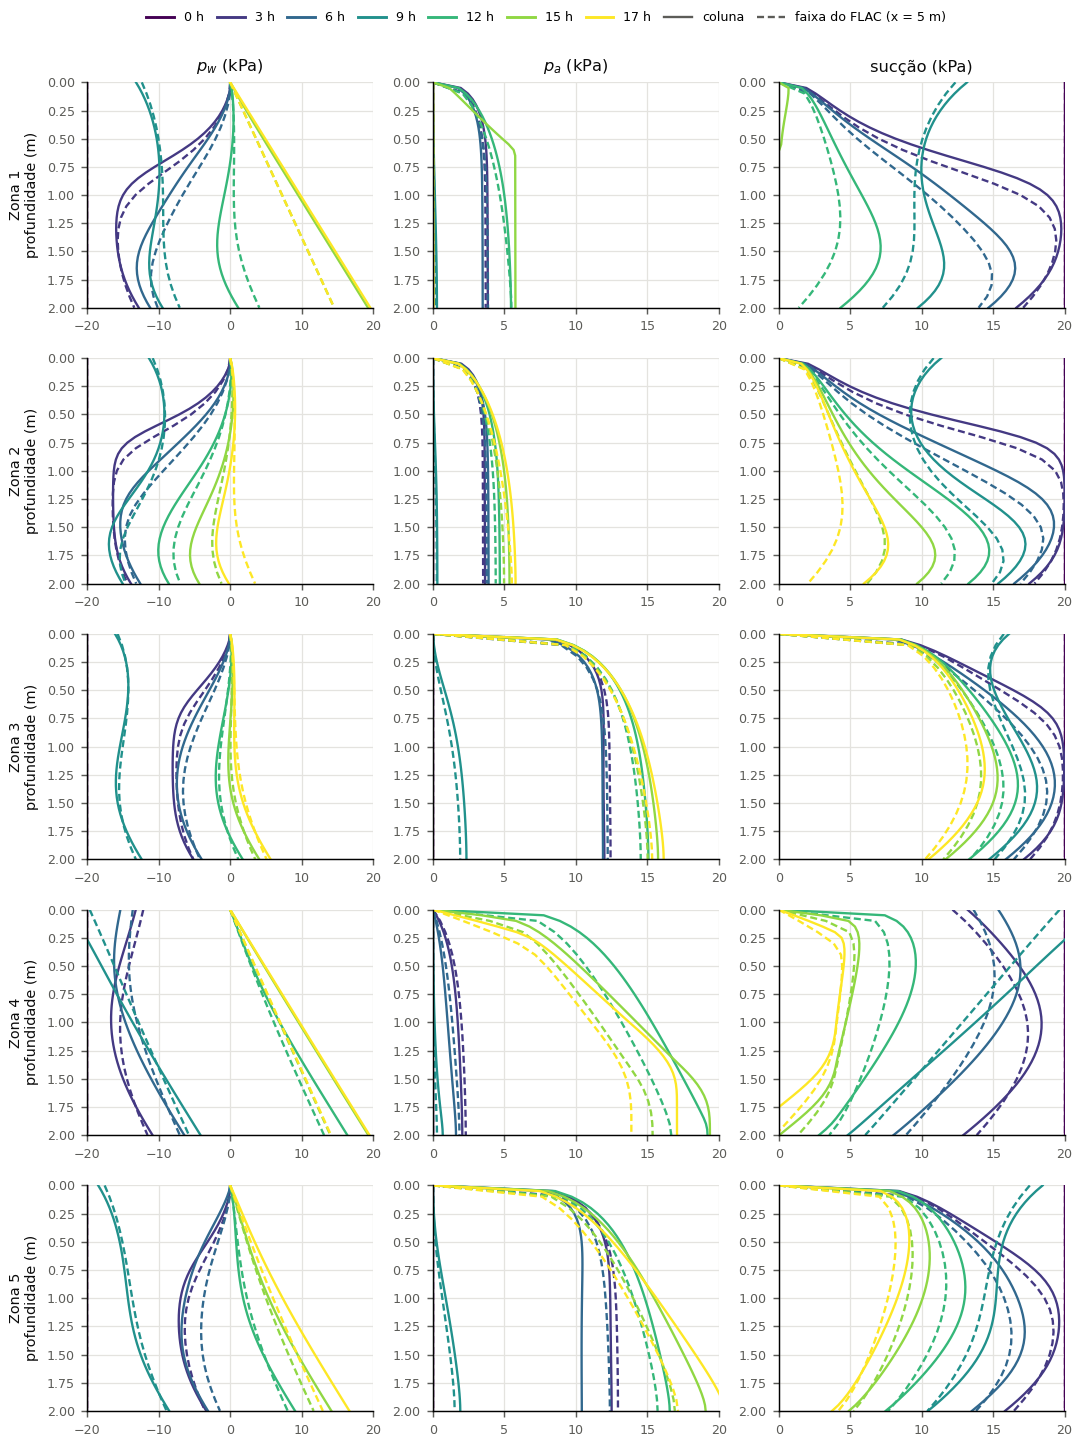
\includegraphics[width=0.85\textwidth]{figs/kang_perfis_tp.png}
\caption{Kang et al.\ (2020), com ar ativo: perfis de $p_w$, $p_a$ e sucção na coluna (linhas cheias) e na faixa do
artigo, na vertical do meio (tracejadas); compare com a Fig.~8 do artigo.}\label{fig:kangperfis}
\end{figure}

\paragraph{Na malha do artigo.} Até a coluna saturar, a faixa e a coluna coincidem, nos dois modelos
(Fig.~\ref{fig:kangfaixacol}): a infiltração é 1D, e a hipótese da coluna vale. Com ar ativo, em que o meio da faixa
não chega a saturar, a faixa acompanha o artigo até o fim (zonas 2, 3 e 5). A diferença aparece depois da saturação
(Tab.~\ref{tab:kangfaixa}):
\begin{itemize}
  \item \textbf{A faixa drena ao longo da encosta.} Saturada, a água escoa paralela ao talude e sai pela superfície na
    parte de baixo; no meio, $p_w$ cai para $\gamma_w z\cos^2\beta$ (75\,\% do hidrostático a $30^\circ$: 13,7~kPa a
    1,9~m, contra 18,6~kPa), e o FS final fica 0,15 a 0,25 acima do da coluna e do artigo. A Eq.~14 com o solo saturado e o $p_w$
    analítico confere: com $\gamma_w z\cos^2\beta$ ela dá o FS final da faixa, e com $\gamma_w z$, o da coluna
    (Tab.~\ref{tab:kangfaixa}); a diferença entre as duas malhas é toda a poropressão do escoamento paralelo.
  \item \textbf{O artigo é hidrostático no fim.} Os perfis finais do artigo (Fig.~8 dele: $\approx 19$~kPa no fundo) e o
    FS final batem com a coluna, não com a faixa: apesar da malha inclinada, os resultados publicados se comportam como
    uma coluna 1D, sem drenagem ao longo da faixa. Provável: o topo do FLAC só recebe a chuva ($q_w = I(t)$), sem saída
    de água, e a faixa enche como um vaso fechado. \afazer{confirmar (o manual do FLAC, ou os autores)}
  \item \textbf{A convenção da chuva.} Com a chuva por metro de superfície inclinada a faixa satura $\approx 1$~h antes
    do artigo ($1/\cos\beta$: 17\,\% mais água a $31^\circ$); a coluna, com a chuva por metro horizontal, acerta a hora.
    Com a chuva por metro horizontal, a faixa satura na mesma hora (abaixo): a convenção pesa pouco.
\end{itemize}
\paragraph{A coluna normal ao talude.} O modelo 1D correto do talude infinito é a coluna com o eixo normal à
superfície: espessura $H\cos\beta$, gravidade $g\cos\beta$ ao longo dela (o peso do solo e os termos de Darcy da água e
do ar) e a chuva vertical como $I\cos\beta$ por metro de superfície; a componente paralela da gravidade fica de fora,
porque no talude infinito o fluxo paralelo é uniforme. Saturada sobre a base impermeável, ela dá
$p_w = \gamma_w z\cos^2\beta$ sem precisar da faixa. Contra a faixa com a mesma chuva (por metro horizontal), o FS final
coincide até a terceira casa nas cinco zonas e nos dois modelos, e ao longo das 17~h a diferença fica abaixo de 0,02,
exceto onde as duas saturam com uma hora de diferença (Tab.~\ref{tab:kangnormal}, Fig.~\ref{fig:kangnormal}); o custo é
o da coluna ($\approx 45$~s contra $\approx 10$~min). Com a chuva por metro horizontal a faixa satura na mesma hora que
com a chuva por metro inclinado: o efeito dominante é a drenagem, não a convenção. A coluna vertical, que reproduz o
artigo, é a mesma coluna sem a drenagem (hidrológicamente um terreno plano) e subestima o FS depois da saturação.

\begin{table}[H]\centering\small
\caption{Kang et al.\ (2020): o FS final (17~h) no ângulo médio na coluna normal ao talude, na faixa do artigo com a chuva
por metro horizontal, na coluna vertical e no artigo; e a maior diferença entre a coluna normal e a faixa ao longo das
17~h.}\label{tab:kangnormal}
\begin{tabular}{cc|cccc|c}
\toprule
zona & modelo & coluna normal & faixa & coluna vertical & Kang & $\max|\Delta|$ normal--faixa\\
\midrule
1 & SP & 0{,}95 & 0{,}95 & 0{,}81 & 0{,}82 & 0{,}00 \\
1 & TP & 0{,}95 & 0{,}95 & 0{,}81 & 0{,}82 & 0{,}00 \\
2 & SP & 0{,}79 & 0{,}79 & 0{,}63 & 0{,}62 & 0{,}00 \\
2 & TP & 1{,}16 & 1{,}15 & 1{,}24 & 1{,}05 & 0{,}00 \\
3 & SP & 1{,}07 & 1{,}07 & 0{,}83 & 0{,}79 & 0{,}02 \\
3 & TP & 1{,}49 & 1{,}49 & 1{,}46 & 1{,}38 & 0{,}01 \\
4 & SP & 0{,}91 & 0{,}91 & 0{,}73 & 0{,}72 & 0{,}19 \\
4 & TP & 0{,}92 & 0{,}92 & 0{,}73 & 0{,}72 & 0{,}04 \\
5 & SP & 0{,}81 & 0{,}81 & 0{,}65 & 0{,}60 & 0{,}00 \\
5 & TP & 0{,}86 & 0{,}86 & 0{,}74 & 0{,}68 & 0{,}00 \\
\bottomrule
\end{tabular}

\end{table}

\begin{figure}[H]\centering
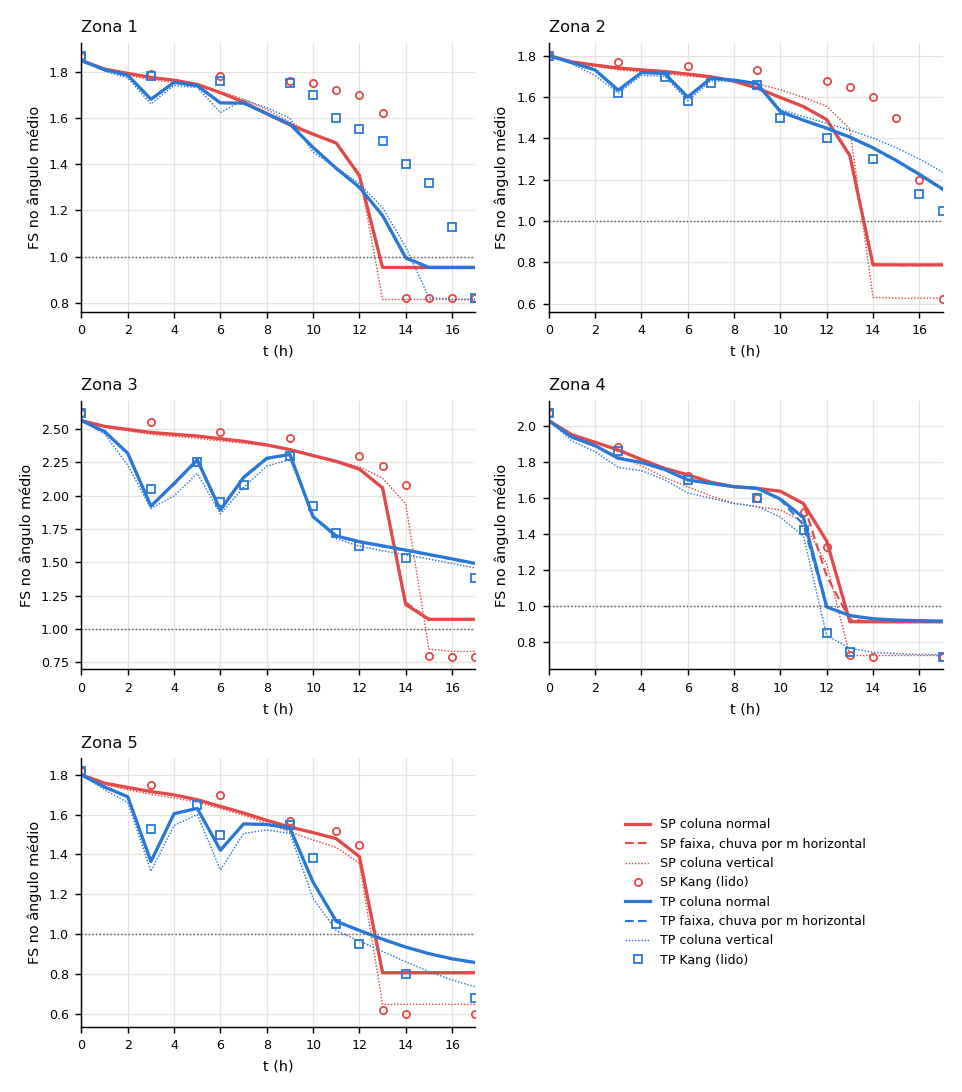
\includegraphics[width=0.9\textwidth]{figs/kang_normal.png}
\caption{Kang et al.\ (2020): FS no ângulo médio na coluna normal ao talude (cheia), na faixa com a chuva por metro
horizontal (tracejada, coberta pela cheia), na coluna vertical (pontilhada) e no artigo (marcadores).}\label{fig:kangnormal}
\end{figure}

Para este artigo, a drenagem ao longo da encosta é um efeito de primeira ordem no FS depois da saturação; no talude 2D
de Rahardjo ela entra naturalmente (o fluxo é resolvido no talude inteiro).

\begin{figure}[H]\centering
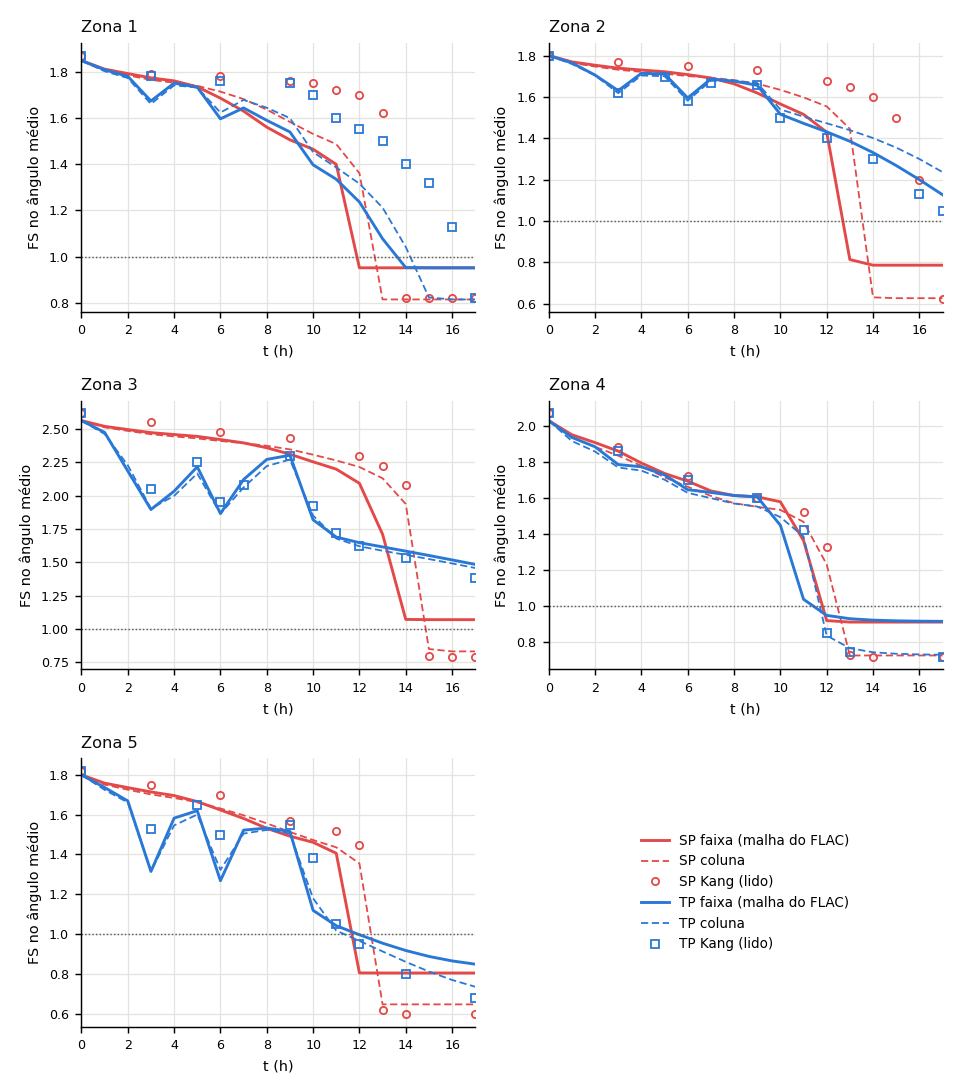
\includegraphics[width=0.9\textwidth]{figs/kang_faixa_coluna.png}
\caption{Kang et al.\ (2020): FS no ângulo médio de cada zona na faixa do artigo (linhas cheias), na coluna
(tracejadas) e no artigo (marcadores, lidos da Fig.~9), sem ar (SP, vermelho) e com ar ativo (TP, azul).}\label{fig:kangfaixacol}
\end{figure}

\begin{table}[H]\centering\small
\caption{Kang et al.\ (2020): o FS final (17~h) no ângulo médio de cada zona, na faixa do artigo, na coluna e no artigo
(lido da Fig.~9, $\pm 0{,}05$). Conferência: a Eq.~14 com o solo saturado ($S_w = 1$, $W$ da Eq.~15) e $p_w$ analítico,
o do escoamento paralelo ao talude ($\gamma_w z\cos^2\beta$, a faixa drenando) e o hidrostático ($\gamma_w z$, a coluna
sem drenagem).}\label{tab:kangfaixa}
\resizebox{\textwidth}{!}{\begin{tabular}{c|ccc|ccc|cc}
\toprule
 & \multicolumn{3}{c|}{SP (ar passivo)} & \multicolumn{3}{c|}{TP (ar ativo)} & \multicolumn{2}{c}{Eq.~14 saturado, $S_w = 1$}\\
zona & faixa & coluna & Kang & faixa & coluna & Kang & $p_w = \gamma_w z\cos^2\beta$ & $p_w = \gamma_w z$\\
\midrule
1 & 0{,}95 & 0{,}81 & 0{,}82 & 0{,}95 & 0{,}81 & 0{,}82 & 0{,}95 & 0{,}81 \\
2 & 0{,}79 & 0{,}63 & 0{,}62 & 1{,}13 & 1{,}24 & 1{,}05 & 0{,}79 & 0{,}63 \\
3 & 1{,}07 & 0{,}83 & 0{,}79 & 1{,}48 & 1{,}46 & 1{,}38 & 1{,}07 & 0{,}83 \\
4 & 0{,}91 & 0{,}73 & 0{,}72 & 0{,}92 & 0{,}73 & 0{,}72 & 0{,}91 & 0{,}73 \\
5 & 0{,}81 & 0{,}65 & 0{,}60 & 0{,}85 & 0{,}74 & 0{,}68 & 0{,}81 & 0{,}65 \\
\bottomrule
\end{tabular}
}
\end{table}

